\documentclass[11pt,compress,t,notes=noshow, xcolor=table]{beamer}
\usepackage[]{graphicx}\usepackage[]{color}
% maxwidth is the original width if it is less than linewidth
% otherwise use linewidth (to make sure the graphics do not exceed the margin)
\makeatletter
\def\maxwidth{ %
  \ifdim\Gin@nat@width>\linewidth
    \linewidth
  \else
    \Gin@nat@width
  \fi
}
\makeatother

\definecolor{fgcolor}{rgb}{0.345, 0.345, 0.345}
\newcommand{\hlnum}[1]{\textcolor[rgb]{0.686,0.059,0.569}{#1}}%
\newcommand{\hlstr}[1]{\textcolor[rgb]{0.192,0.494,0.8}{#1}}%
\newcommand{\hlcom}[1]{\textcolor[rgb]{0.678,0.584,0.686}{\textit{#1}}}%
\newcommand{\hlopt}[1]{\textcolor[rgb]{0,0,0}{#1}}%
\newcommand{\hlstd}[1]{\textcolor[rgb]{0.345,0.345,0.345}{#1}}%
\newcommand{\hlkwa}[1]{\textcolor[rgb]{0.161,0.373,0.58}{\textbf{#1}}}%
\newcommand{\hlkwb}[1]{\textcolor[rgb]{0.69,0.353,0.396}{#1}}%
\newcommand{\hlkwc}[1]{\textcolor[rgb]{0.333,0.667,0.333}{#1}}%
\newcommand{\hlkwd}[1]{\textcolor[rgb]{0.737,0.353,0.396}{\textbf{#1}}}%
\let\hlipl\hlkwb

\usepackage{framed}
\makeatletter
\newenvironment{kframe}{%
 \def\at@end@of@kframe{}%
 \ifinner\ifhmode%
  \def\at@end@of@kframe{\end{minipage}}%
  \begin{minipage}{\columnwidth}%
 \fi\fi%
 \def\FrameCommand##1{\hskip\@totalleftmargin \hskip-\fboxsep
 \colorbox{shadecolor}{##1}\hskip-\fboxsep
     % There is no \\@totalrightmargin, so:
     \hskip-\linewidth \hskip-\@totalleftmargin \hskip\columnwidth}%
 \MakeFramed {\advance\hsize-\width
   \@totalleftmargin\z@ \linewidth\hsize
   \@setminipage}}%
 {\par\unskip\endMakeFramed%
 \at@end@of@kframe}
\makeatother

\definecolor{shadecolor}{rgb}{.97, .97, .97}
\definecolor{messagecolor}{rgb}{0, 0, 0}
\definecolor{warningcolor}{rgb}{1, 0, 1}
\definecolor{errorcolor}{rgb}{1, 0, 0}
\newenvironment{knitrout}{}{} % an empty environment to be redefined in TeX

\usepackage{alltt}
\newcommand{\SweaveOpts}[1]{}  % do not interfere with LaTeX
\newcommand{\SweaveInput}[1]{} % because they are not real TeX commands
\newcommand{\Sexpr}[1]{}       % will only be parsed by R



\usepackage[english]{babel}
\usepackage[utf8]{inputenc}

\usepackage{dsfont}
\usepackage{verbatim}
\usepackage{amsmath}
\usepackage{amsfonts}
\usepackage{bm}
\usepackage{csquotes}
\usepackage{multirow}
\usepackage{longtable}
\usepackage{booktabs}
\usepackage{enumerate}
\usepackage[absolute,overlay]{textpos}
\usepackage{psfrag}
\usepackage{algorithm}
\usepackage{algpseudocode}
\usepackage{eqnarray}
\usepackage{arydshln}
\usepackage{tabularx}
\usepackage{placeins}
\usepackage{tikz}
\usepackage{setspace}
\usepackage{colortbl}
\usepackage{mathtools}
\usepackage{wrapfig}
\usepackage{bm}
\usetikzlibrary{shapes,arrows,automata,positioning,calc,chains,trees, shadows}
\tikzset{
  %Define standard arrow tip
  >=stealth',
  %Define style for boxes
  punkt/.style={
    rectangle,
    rounded corners,
    draw=black, very thick,
    text width=6.5em,
    minimum height=2em,
    text centered},
  % Define arrow style
  pil/.style={
    ->,
    thick,
    shorten <=2pt,
    shorten >=2pt,}
}
\usepackage{subfig}


% Defines macros and environments
\input{../../style/common.tex}
% \input{common.tex}

%\usetheme{lmu-lecture}
\newcommand{\titlefigure}{figure/eval_train_2}
\newcommand{\learninggoals}{
\item Understand the definition of training error
\item Understand why training error is no reliable estimator of future performance}
\usepackage{../../style/lmu-lecture}


%\usetheme{lmu-lecture}
\usepackage{../../style/lmu-lecture}

\let\code=\texttt
\let\proglang=\textsf

\setkeys{Gin}{width=0.9\textwidth}

\title{Introduction to Machine Learning}
% \author{Bernd Bischl, Christoph Molnar, Daniel Schalk, Fabian Scheipl}
\institute{\href{https://compstat-lmu.github.io/lecture_i2ml/}{compstat-lmu.github.io/lecture\_i2ml}}
\date{}

\setbeamertemplate{frametitle}{\expandafter\uppercase\expandafter\insertframetitle}

\begin{document}

% This file loads R packages, configures knitr options and sets preamble.Rnw as parent file
% IF YOU MODIFY THIS, PLZ ALSO MODIFY setup.Rmd ACCORDINGLY...

% Defines macros and environments
\input{../../latex-math/basic-math.tex}
\input{../../latex-math/basic-ml.tex}

%! includes: evaluation-intro 

\lecturechapter{Evaluation: Training Error}
\lecture{Introduction to Machine Learning}

% ------------------------------------------------------------------------------

\begin{vbframe}{Training Error}

The \textbf{training error} (also called apparent error or resubstitution error)
is estimated by averaging the errors over the training observations that have 
been used to fit the model:

\vfill

\begin{center}
% FIGURE SOURCE: https://docs.google.com/drawings/d/1m0Uwf5bvWuP1agyZ0TOd0qaBakJVtfe_PspxqPL3mxU/edit?usp=sharing
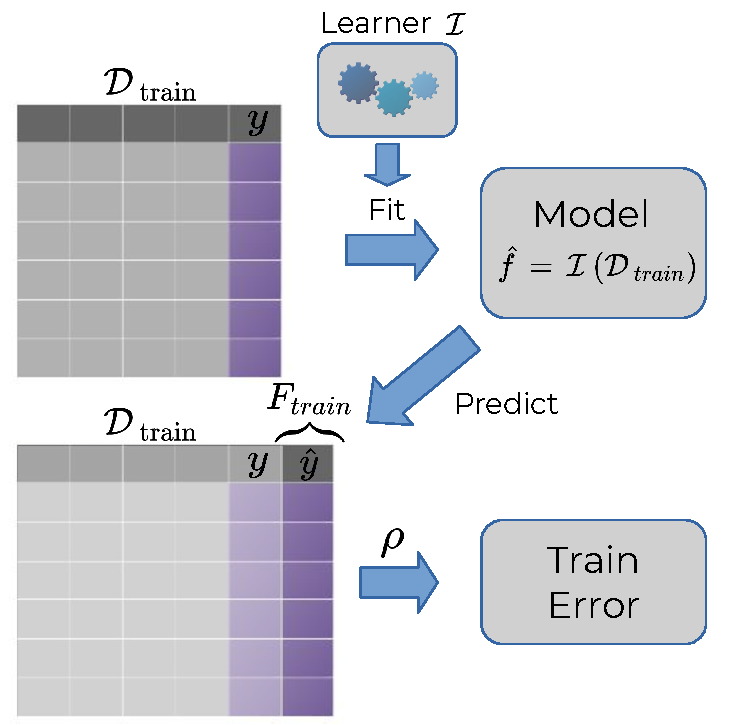
\includegraphics[width=.55\textwidth]{figure_man/train_error.pdf}
\end{center}

\end{vbframe}

% ------------------------------------------------------------------------------

\begin{vbframe}{Example: Polynomial Regression}

Sample data from sinusoidal function
$0.5 + 0.4 \cdot \sin (2 \pi x) + \epsilon$\\
with measurement error $\epsilon$:

\vfill

\begin{center}
  \includegraphics[width=0.85\textwidth]{figure/eval_train_1}
\end{center}

Now assume the data-generating process to be unknown as usual.\\
Try to approximate the data with a $d^{th}$-degree polynomial:
\[ \fxt = \theta_0 + \theta_1 \xv + \cdots + \theta_d \xv^d = \sum_{j = 0}^{d}
\theta_j \xv^j\text. \]

\framebreak

Different polynomial orders give rise to models of varying \textbf{complexity}.
$\rightarrow$ How to choose $d$?

\vfill

\begin{minipage}[c]{0.6\textwidth}
  % \centering
  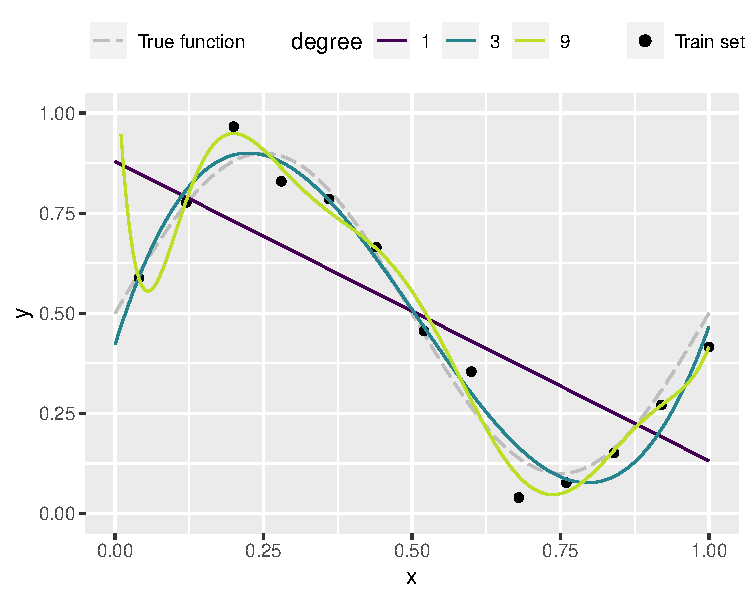
\includegraphics[width=\textwidth]{figure/eval_train_2} 
\end{minipage}%
\begin{minipage}[c]{0.4\textwidth}
  \begin{itemize}
    \footnotesize
    \item $d = 1$: MSE = 0.036: \\clearly underfitting
    \item $d = 3$: MSE = 0.003: \\pretty OK
    \item $d = 9$: MSE = 0.001: \\clearly overfitting
  \end{itemize}
\end{minipage}

\vfill

$\rightarrow$ Choosing $d$ based on minimal training error seems to be a bad 
idea.

\end{vbframe}

% ------------------------------------------------------------------------------

\begin{vbframe}{Training Error Problems}

\begin{itemize}
  \item The training error is an unreliable and \textbf{optimistically biased} 
  estimator of future performance. \\
  $\rightarrow$ Extreme example: training error of 1-NN is always 0 as each 
  observation is its own NN at test time.
  \item We are interested in modeling the inherent data structure, not in 
  fitting every peculiarity or noise in the training data.
  \item \textbf{Goodness-of-fit} measures like (classic) $R^2$, likelihood, AIC, 
  BIC, deviance are all based on the training error.
  \item For models of restricted capacity, and given enough data, the training 
  error may provide reliable information.
  \begin{itemize}
    \item E.g., for a linear model with 5 features and $10^6$ training points.
    \item \textbf{But:} it is impossible to know when the training error starts 
    to become unreliable.
  \end{itemize}
  % \item \textcolor{blue}{Extend any ML training in the following way:
  %   After normal fitting, we also store the training data.
  %   During prediction, we first check whether $x$ is already stored in this set. 
  %   If so, we replicate its label.
  %   The train error of such an (unreasonable) procedure will be 0.}
  % \item \textcolor{blue}{There are so called interpolators - interpolating 
  % splines, interpolating Gaussian processes - whose predictions can always 
  % perfectly match the regression targets, they are not necessarily good as they 
  % will interpolate the noise too.}
\end{itemize}
\end{vbframe}

% ------------------------------------------------------------------------------

\begin{vbframe}{training error and generalization}

\begin{minipage}[c]{0.6\textwidth}
  \small
  We simulate 100,000 points from the \texttt{spirals} data with $sd = 0.1$ and 
  train a $k$-nearest neighbor classifier with $k$ set to 15.
\end{minipage}%
\begin{minipage}[c]{0.05\textwidth}
  \phantom{foo}
\end{minipage}%
\begin{minipage}[c]{0.35\textwidth}
  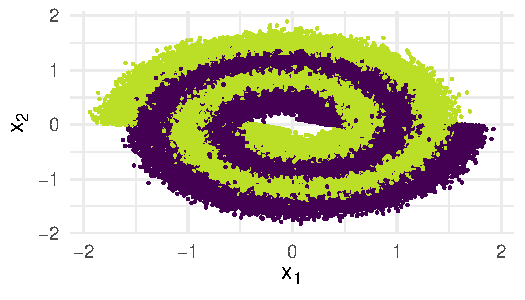
\includegraphics[width = 0.9\textwidth]{figure/eval_delta_train_test_err_data}
\end{minipage}%

\vfill

\small

For a sufficient amount of training data the training error should yield a 
fairly good indication of the true generalization ability.

\vfill

We set aside a very large test set of 70,000 observations to gauge the true 
generalization error as well as possible.
Steadily increasing the training set size from 16 to 30,000 data points, we 
observe how the gap between training and test error narrows and bottoms 
out close to 0:

\vfill

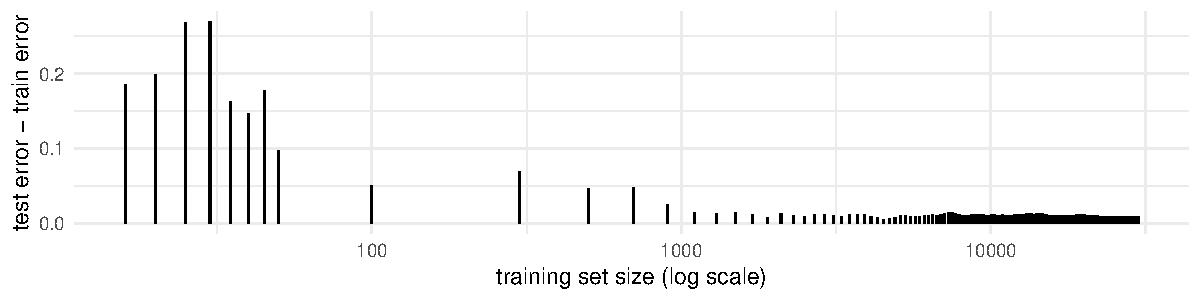
\includegraphics[width = \textwidth]{figure/eval_delta_train_test_err}

\framebreak

% ------------------------------------------------------------------------------

\small

The example suggests that, for a large amount of training data and a rather
simple learner, the training error can hold quite reliable information about 
the learner's ability to generalize.

\vfill

\textbf{But:} assuming a more realistic scenario with a total of 500 training
observations (while the test set remains the same) and allowing for more 
complexity, the picture changes:

\vfill

\begin{center}
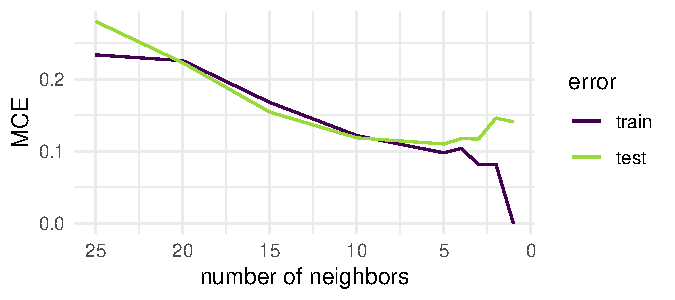
\includegraphics[width = 0.7\textwidth]{figure/eval_delta_train_test_overfit}
\end{center}

\vfill

The low training error for small $k$ is deceptive -- as the model becomes more 
and more local, test error starts creeping up as the learner fits the 
training data very closely at the expense of generalization.

\end{vbframe}

% ------------------------------------------------------------------------------

\endlecture
\end{document}
